\section{Результаты}
\label{sec:Results} \index{Chapter6}

\subsection{Результаты русскоязычной адаптации}
\label{subsec:mmlu_results} \index{Chapter6!mmlu_results}

\begin{table}[ht]
\centering
\caption{MMLU accuracy}
\fontsize{12}{14}\selectfont
\renewcommand{\arraystretch}{1.2}
\begin{tabularx}{\textwidth}{
  >{\centering\arraybackslash}p{6cm} 
  >{\centering\arraybackslash}p{4cm} 
  >{\centering\arraybackslash}p{4cm}
}
\toprule
\textbf{Model} & \textbf{Default} & \textbf{RU Finetune} \\
\midrule
Qwen2.5-1.5B Instruct & 39.36\% & 42.14\% \\
\midrule
Qwen2.5-3B Instruct & 47.96\% & 49.55\% \\
\bottomrule
\end{tabularx}
\end{table}

По метрикам на MMLU виден прирост, однако дальнейшее обучение этих моделей на WebGLM показало существенное ухудшение итогового качества для Qwen2.5-1.5B Instruct --- доля верных ответов на бенчмарке упала на 5-10\%. Вероятно это связано с тем, что модель переобучалась под формат данных и начинала хуже работать с контекстной информацией. Для Qwen2.5-3B Instruct падение было не столь существенно, но итоговое качество так же не улучшилось. В целом можно сказать, что этот этап необходим только для моделей, плохо работающих с русскоязычными текстами.



\subsection{Результаты WebGLM и RAFT}
\label{subsec:webglm_results} \index{Chapter6!webglm_results}

\begin{figure}[ht!]
    \centering
    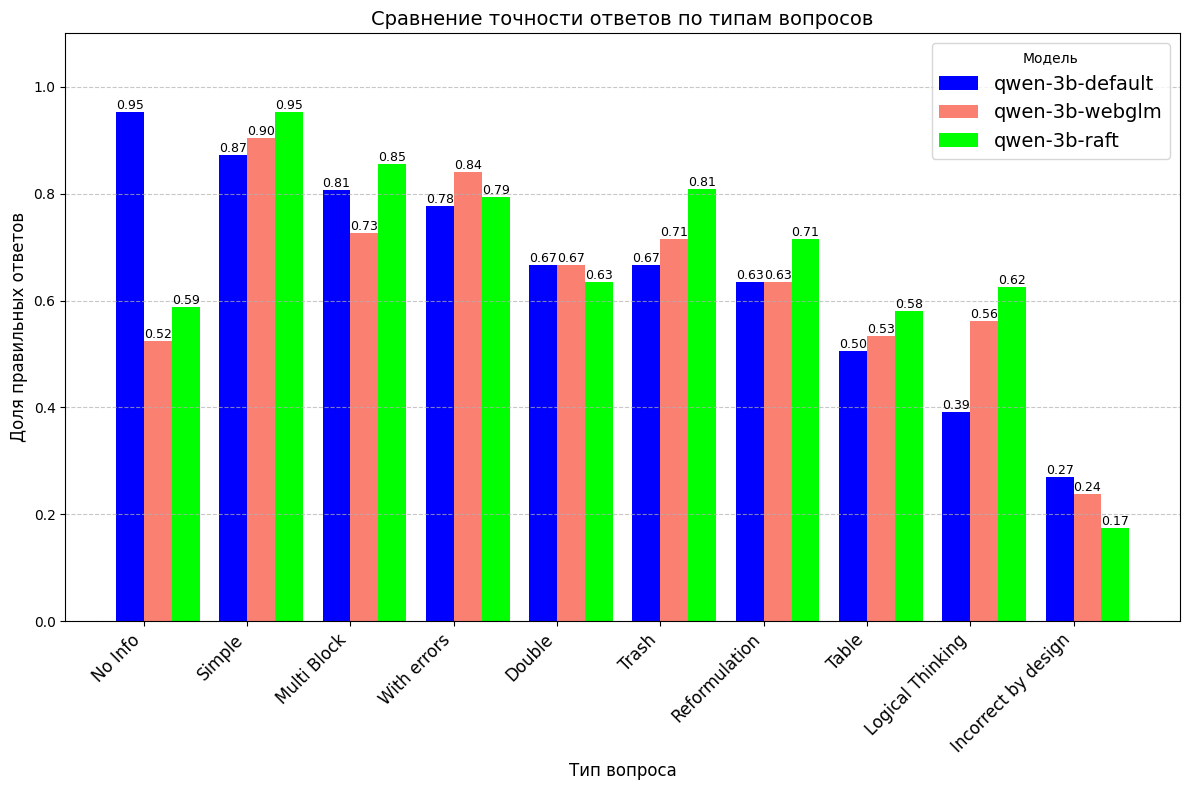
\includegraphics[scale=0.5]{images/3b_raft_result.png}
    \label{RAFT 3b}
\end{figure}

Можно заметить существенный рост качества RAFT на всех типах вопросов, кроме <<No Info>> и <<Incorrect by design>>. Важно отметить, что снижение качества ответа на <<No Info>> связо в первую очередь со снижение доли шаблонных отказов при ответах.

\textbf{Доля отказов}: 
\begin{itemize}
    \item Default - 30\% (из них 70\% неуместно).

    \item WebGLM - 9\% (из них 49\% неуместно).

    \item RAFT - 8\% (из них 36\% неуместно).
\end{itemize}

По результатам обучения 1.5B моделей так же был получен прирост, однако в данном случае метод RAFT показал себя хуже. Вероятно такого количества параметров недостаточно для качественной работы модели на этой задаче.

\begin{figure}[ht!]
    \centering
    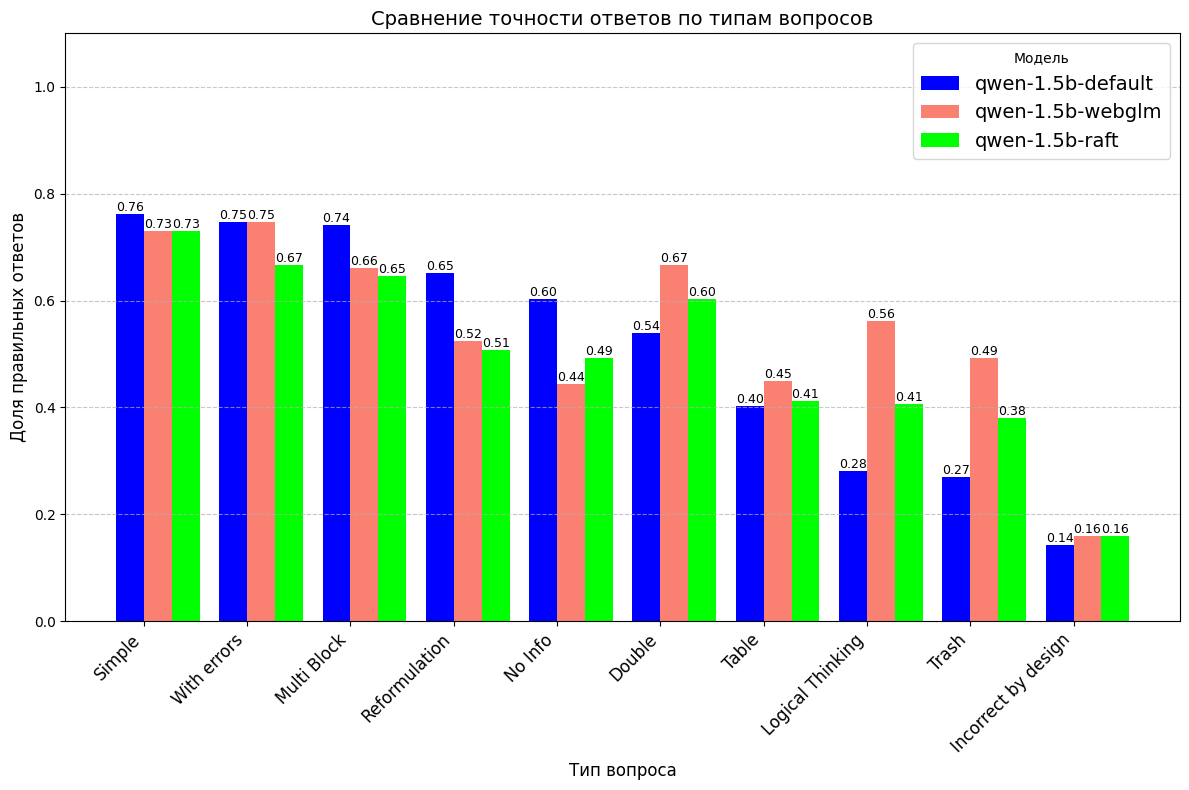
\includegraphics[scale=0.5]{images/1_5b_raft_result_new.png}
    \label{RAFT 1.5b}
\end{figure}

В целом можно увидеть преимущество обучения RAFT относительно классического finetune на WebGLM для среднего размера моделях. Этот этап крайне эффективен и не требует дополнительных модификаций. Итоговые метрики можно увидеть в сводных таблицах:  

\begin{table}[h]
\centering
\caption{\textit{Оценки LLM.}}
\renewcommand{\arraystretch}{1.0}  % Increase row spacing
\begin{tabular}{@{}lcccc@{}}
\toprule
\textbf{Model} & \textbf{AVG Score} & \textbf{Accuracy} & \textbf{Irrelevant Refuse} \\
\midrule
Qwen2.5-1.5b-default        & 3.31              & 0.50                & 0.18             \\
Qwen2.5-1.5b-WebGLM       & \textbf{3.37}      & \textbf{0.53}      & \textbf{0.06}             \\
Qwen2.5-1.5b-RAFT        & 3.32              & 0.50                & 0.15             \\
Qwen2.5-3b-default          & 3.86     & 0.64                & 0.21             \\
Qwen2.5-3b-WebGLM       & 3.73              & 0.63                & 0.05             \\
Qwen2.5-3b-RAFT         & \textbf{3.86}     & \textbf{0.67}       & \textbf{0.03}    \\
Qwen2.5-32b-default       & 4.28            & 0.77                      & 0.12    \\
\bottomrule
\end{tabular}
\end{table}

\begin{table}[h]
\centering
\caption{\textit{ROUGE-L метрики.}}
\renewcommand{\arraystretch}{1.0}  % Increase row spacing
\begin{tabular}{@{}lcccc@{}}
\toprule
\textbf{Model} & \textbf{Precision} & \textbf{Recall} & \textbf{F1}\\
\midrule
Qwen2.5-1.5b-default        & 0.18              & 0.34                & 0.20             \\
Qwen2.5-1.5b-WebGLM        & \textbf{0.19}       & 0.36        & \textbf{0.22}             \\
Qwen2.5-1.5b-RAFT        & 0.14              & \textbf{0.40}                & 0.19             \\
Qwen2.5-3b-default          & 0.18              & 0.40                & 0.23             \\
Qwen2.5-3b-WebGLM       & \textbf{0.23}     & 0.41                & \textbf{0.27}    \\
Qwen2.5-3b-RAFT         & 0.14              & \textbf{0.51}       & 0.20             \\
Qwen2.5-32b-default       & 0.36            & 0.53                      & 0.40    \\
\bottomrule
\end{tabular}
\end{table}


\newpage

\subsection{<<Lost in the middle>> и синтетические данные}
\label{subsec:synth_results} \index{Chapter6!synth_results}

Для исследования актуальности проблемы <<lost in the middle>> были проведены замеры на срезке из 231 примера бенчмарка с разным количеством документов и их положениями в контексте.

\begin{table}[h]
\centering
\caption{\textit{Качество Qwen2.5-3b-default при разных положениях документов, метрика - среднее значение accuracy.}}
\renewcommand{\arraystretch}{1.0}  % Increase row spacing
\begin{tabular}{@{}lcccc@{}}
\toprule
\textbf{Documents} & \textbf{Default order} & \textbf{Reverse order} & \textbf{Random shuffle}\\
\midrule
Top-5 (2k context)       & \textbf{0.68}     & 0.64       & \textbf{0.68}                \\
Top-10 (4k context)         & \textbf{0.72}     & 0.71       & 0.68                \\
Top-20 (8k context)        & 0.68              & 0.68       & \textbf{0.71}       \\
\bottomrule
\end{tabular}
\end{table}

Можно сделать вывод, что на таком размере контекста у современных моделей нет явно выраженного эффекта <<lost in the middle>>, а также количество документов имеет слабое влияние на результат при достаточно качественной retriever модели (в данном случае $recall@10 > 0.9$). Дообучение на синтетике так же не привело к росту качества на бенчмарке, а потому расценено как неактуальное.

\newpage
